\newcommand{\ClassPath}{../../VIU_TFM_LaTeX_template}
\documentclass{\ClassPath/viu-tfm-template}
\usepackage{multicol}

\definecolor{maincolor}{HTML}{f25416}

%--------------------------------------------------------------------------
% Definiciones necesarias Modifica con tus datos
%--------------------------------------------------------------------------
\def\nombre{Gómez Olivencia, Rubén}
\def\dni{78910013-A}
\def\titulo{Cuadro de mandos \linebreak\linebreak con OpenData Euskadi}
\def\titulacion{Máster Universitario en Desarrollo de Aplicaciones y Servicios Web}
\def\curso{2022-2023}

%Los siguientes son opcionales: si no se ponen, la portada cambia un poco. Ideal para escribir artículos/trabajos cortos
\def\dirige{}
\def\convocatoria{}
\def\asignatura{Análisis de datos Web}


% importar fichero de Bibliografía
%\addbibresource{Actividad_1.bib}

\begin{document}
    \graphicspath{{../../VIU_TFM_LaTeX_template/}}

    \coverpage

    \tableofcontents

\chapter{Introducción}

A la hora de realizar un análisis de datos (del tipo que sean, datos web, científicos, logs informáticos, meteorológicos, ...) no sólo es importante el propio análisis realizado y la información obtenida, sino que también es importante cómo se muestra esa información.

El aspecto que le damos a esa información, junto con la posibilidad de interactuar con ella, puede hacer que esa información llegue a más gente y que se entienda de mejor manera que si sólo es plasmada sin ningún tipo de cuidado.

En este documento se va a explicar cómo se ha realizado la obtención de datos de eventos culturales obtenidos de la web OpenData del Gobierno Vasco, el análisis y procesado realizado, y cómo se ha creado un cuadro de mandos con la información obtenida.

\chapter{Contexto de uso}

Hoy en día se suelen realizar muchos eventos culturales pero que quizá no conozcamos porque no se les ha dado la propaganda suficiente al ser un evento pequeño o por tratarse de un evento en una localidad que no es la nuestra.

Para evitar eso, desde el departamento de datos abiertos \href{https://www.opendata.euskadi.eus/inicio/}{Open Data Euskadi} han creado una API asociada a eventos culturales a la que se puede solicitar datos desde la siguiente \href{https://www.opendata.euskadi.eus/api-culture/?api=culture_events}{url}.

Aunque existe una web para realizar consultas de los próximos eventos, no se pueden consultar datos anteriores a la fecha actual, a modo de histórico, o para tener un agregado de datos.

Es por eso que a través del \href{https://datastudio.google.com/reporting/2322c44e-ad75-4243-a4a5-257be6d754bf/page/9AT6C}{cuadro de mandos} que se ha realizado, se puede obtener dicha información, ya sea pasada, presente o futura (teniendo en cuenta los datos existentes).


\chapter{Datos obtenidos y análisis realizado}

A continuación se va a exponer todo el proceso de obtención de datos, el análisis realizado y las modificaciones que ha habido que efectuar en parte de los datos.

\section{Fuente de datos}
Tal como se ha dicho previamente, la fuente de datos ha sido el portal \href{https://www.opendata.euskadi.eus/inicio/}{Open Data Euskadi}, concretamente la sección creada para la \href{https://www.opendata.euskadi.eus/api-culture/?api=culture_events}{API de eventos}.

Desde esta web se explica cómo realizar consultas a la API y para ello se ha hecho uso del comando \commandbox{curl} para realizar la siguiente consulta y obtención de datos.

\begin{mycode}{Extracción de datos}{console}{{\small }}
ruben@vega ~$ curl -X GET \
  "https://api.euskadi.eus/culture/events/v1.0/events?_elements=5000" \
  -H "accept: application/json" > eventos.json
\end{mycode}

De esta manera hemos obtenido un fichero \configfile{eventos.json} con los 5000 registros que la API nos devuelve, a los que hay que realizar un análisis de lo obtenido.


\section{Análisis y transformación de datos}
Tras obtener los datos, es momento de realizar un análisis del fichero obtenido. Dado que es un fichero \textbf{json}, es fácilmente parseable mediante el lenguaje de programación \href{URLhttps://www.python.org/}{Python}.

En primer lugar es obtener los items de los eventos, ya que la consulta devuelve los datos con la siguiente estructura:

\begin{mycode}{Estructura de datos original}{json}{}
{
    "totalItems": 5000,
    "totalPages": 1,
    "currentPage": 1,
    "items": [
    {
        ...
    }]
}
\end{mycode}

Tras esto, ya podemos recorrer los datos, quedarnos con los índices que nos interesan y comenzar a realizar ciertas modificaciones necesarias. Para ello, se ha tenido que recorrer todos los items de la siguiente manera:

\begin{mycode}{Parte del script de parseo de datos}{python}{}
#!/usr/bin/env python3
import pandas as pd
import json
import re
from datetime import datetime
# ...
for item in items:
    o = json.loads('{}')
    o.update({"Nombre":re.sub('\"','',item['nameEs'].title())})
    o.update({"Tipo":item['typeEs']})
\end{mycode}

Dado que no nos interesan todos los índices de los datos obtenidos, se ha creado una variable “\textbf{o}” donde se irán añadiendo los índices y de paso poniendo un nombre adecuado.

Los dos primeros campos son el nombre y el tipo de evento, que debido a que en los datos obtenidos también hay versión en euskera, tienen un nombre indicando el idioma. Esto ha habido que hacerlo con otros campos como son el precio y el municipio.

Por otro lado, también ha habido que realizar modificaciones en las fechas y con la posición de geolocalización:


\begin{mycode}{Parte del script de parseo de datos}{python}{{\footnotesize }}
d = re.sub('T.*','',item['startDate'])
d = re.sub('-','',d)
o.update({"Fecha inicio":d})
d = re.sub('T.*','',item['endDate'])
d = re.sub('-','',d)
o.update({"Fecha fin":d})
if 'municipalityLatitude' in item and 'municipalityLongitude' in item:
    o.update({"GPS":item['municipalityLatitude']+','+item['municipalityLongitude']})
\end{mycode}

En el caso de las fechas, dado que \href{https://datastudio.google.com/}{Data Studio} no identificaba de manera correcta las fechas, ha habido que convertirlas al formato \textbf{20221103}, donde el año, mes y día está todo junto y en ese orden.

En lo que se refiere a la \textbf{geolocalización}, en los datos se obtenían la latitud y la longitud por separado, y se ha creado un índice juntando ambos datos, para que después pueda ser utilizado.


También ha habido que realizar modificaciones en lo que se refiere a la provincia, ya que en los datos no se obtenía el nombre, sino que aparecía el código de la misma. En la propia API hay otro apartado donde se puede obtener una relación del código con el nombre. Con esa información se ha decidido realizar el siguiente código para hacer los cambios necesarios:

\begin{mycode}{Parte del script de parseo de datos}{python}{}
if item['provinceNoraCode'] == '48':
    o.update({'Provincia':'Bizkaia'})
if item['provinceNoraCode'] == '1':
    o.update({'Provincia':'Araba'})
if item['provinceNoraCode'] == '20':
    o.update({'Provincia':'Gipuzkoa'})
if item['provinceNoraCode'] == '31':
    o.update({'Provincia':'Navarra'})
if item['provinceNoraCode'] == '-3':
    o.update({'Provincia':'Iparralde'})
\end{mycode}


Ha habido algún pequeño otro cambio que ha habido que realizar, pero debido a que son similares a los casos expuestos previamente, se consideran irrelevantes en el ámbito general.

Para finalizar con los datos, cada nuevo evento se ha añadido a un json de eventos (llamado “out”) y que posteriormente se ha convertido a formato \textbf{CSV} a través de la librería \href{https://pandas.pydata.org/}{Pandas}.

\begin{mycode}{Parte del script de parseo de datos}{python}{}
df = pd.read_json(json.dumps(out),dtype=True)
df.to_csv('eventos.csv', index=False)
\end{mycode}

De esta manera tenemos un nuevo fichero \configfile{eventos.csv} que podemos cargar como fuente de datos en \href{https://datastudio.google.com/}{Data Studio}.

\section{Modelo de datos resultante}

Tras la transformación realizada en el paso previo, el modelo resultante de datos (que ha sido exportado a formato CSV) es el siguiente:

\begin{itemize}
    \item \textbf{Nombre}: Nombre del evento en formato texto.
    \item \textbf{Tipo}: Tipo de evento, en formato texto.
    \item \textbf{Fecha inicio}: Fecha de comienzo del evento, en el formato de fecha admitido por Data Studio.
    \item \textbf{Fecha fin}: Fecha de finalización del evento, en el formato de fecha admitido por Data Studio.
    \item \textbf{GPS}: La latitud y la longitud de la geolocalización del evento.
    \item \textbf{Municipio}: El municipio donde se celebra el evento, en formato texto.
    \item \textbf{Idioma}: En caso de que exista el idioma, aparece en formato ISO (EU, ES, ...)
    \item \textbf{Precio}: Dado que en los datos originales es un campo de texto, donde no se sigue una estructura fija de parseo, se mantiene en formato texto.
    \item \textbf{Provincia}: Provincia donde se realiza el evento.
\end{itemize}


\chapter{Creación del cuadro de mandos}

Para crear el \href{https://datastudio.google.com/reporting/2322c44e-ad75-4243-a4a5-257be6d754bf/page/9AT6C}{cuadro de mandos} se ha hecho uso de la aplicación \href{https://datastudio.google.com/}{Data Studio} de Google, ya que nos va a permitir realizar gráficas y mostrar la información de manera sencilla, pero con gran versatilidad.

\section{Carga de datos}
Para poder hacer uso de los datos que previamente se han transformado, hay que realizar la carga en Data Studio. Como ya se ha dicho previamente, el último paso ha sido generar un fichero CSV ya que es uno de los formatos aceptados por la aplicación.

Tras la carga, y haber indicado que el índice GPS es sirve para gelocalización, obtenemos el siguiente resultado:

\begin{center}
    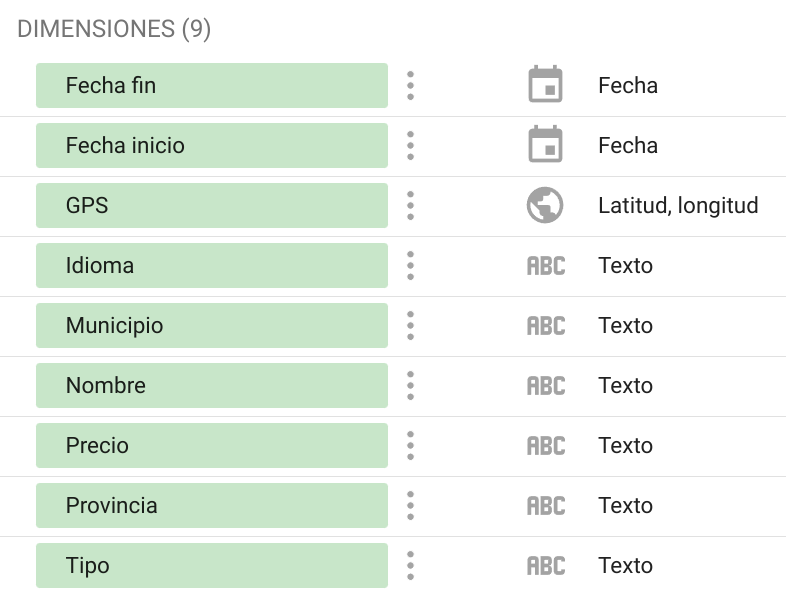
\includegraphics[width=0.6\linewidth]{img/datos.png}
\end{center}

\section{Secciones}

El \href{https://datastudio.google.com/reporting/2322c44e-ad75-4243-a4a5-257be6d754bf/page/9AT6C}{cuadro de mandos} realizado se puede dividir en distintas secciones, con sus correspondientes gráficas que pasaremos a detallar a continuación.


\subsection{Conjunto completo de datos}

La primera sección se hace uso del conjunto completo de datos, en el que se puede ver el total de los datos, elegir por el tipo de evento, el territorio donde se realiza o elegir entre las fechas en las que se realiza.

En caso de realizar alguna modificación en estos controles, se verá reflejado en la tabla que hay a continuación, así como en las gráficas creadas.

Estas gráficas representan:
\begin{itemize}
    \item \textbf{Geoposición de los eventos}: La posición geográfica de los eventos, diferenciando cada tipo de evento con un color distinto.
    \begin{center}
        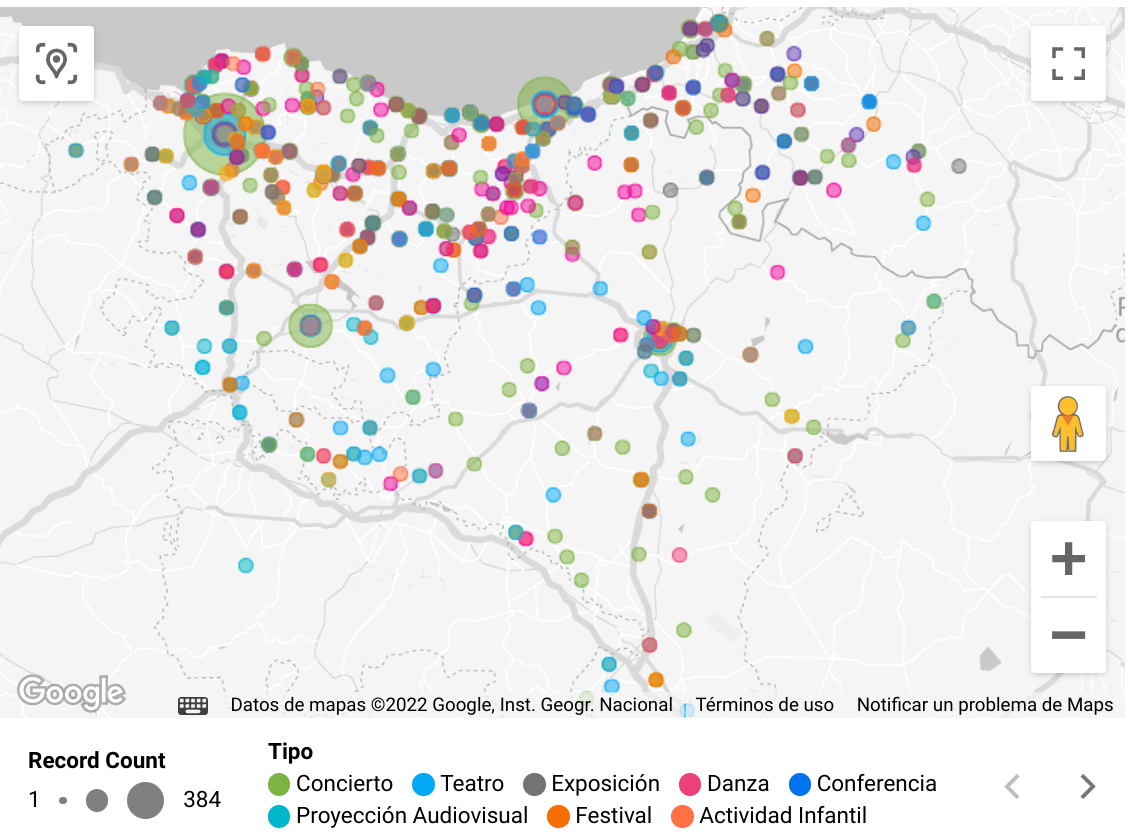
\includegraphics[width=0.6\linewidth]{img/mapa1.png}
    \end{center}

    \item \textbf{Porcentaje de tipos de eventos} en formato de círculo, donde se ve que el mayor porcentaje de eventos son conciertos.
    \begin{center}
        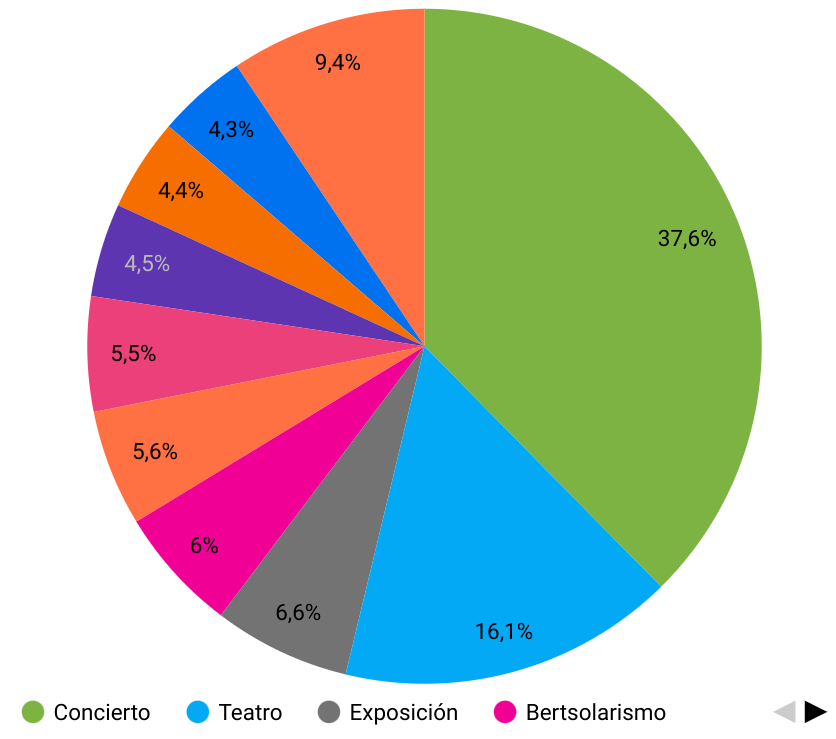
\includegraphics[width=0.6\linewidth]{img/circulo.png}
    \end{center}

    \item \textbf{Mapa de calor} de los eventos. Similar al mapa comentado previamente, pero esta vez en formato de calor.

    \item \textbf{Gráfica de barras} donde aparece que el territorio que más eventos tiene es Bizkaia seguido de Gipuzkoa con mucha diferencia respecto al resto.
\end{itemize}

\subsection{Eventos esta semana}

Se ha decidido crear una sección donde los datos cuenten con un periodo predeterminado, para que las gráficas resultantes sólo muestren la cantidad de eventos que se van a realizar la semana en curso en la que nos encontramos.

\begin{center}
    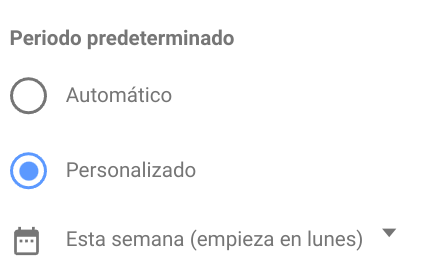
\includegraphics[frame,width=0.3\linewidth]{img/periodo.png}
\end{center}

Hay dos gráficas:

\begin{itemize}
    \item \textbf{Eventos totales} por día de la semana.
    \item \textbf{Eventos diferenciando el territorio}. De esta manera, se puede elegir sólo los eventos del territorio que nos interese.
\end{itemize}

\begin{center}
    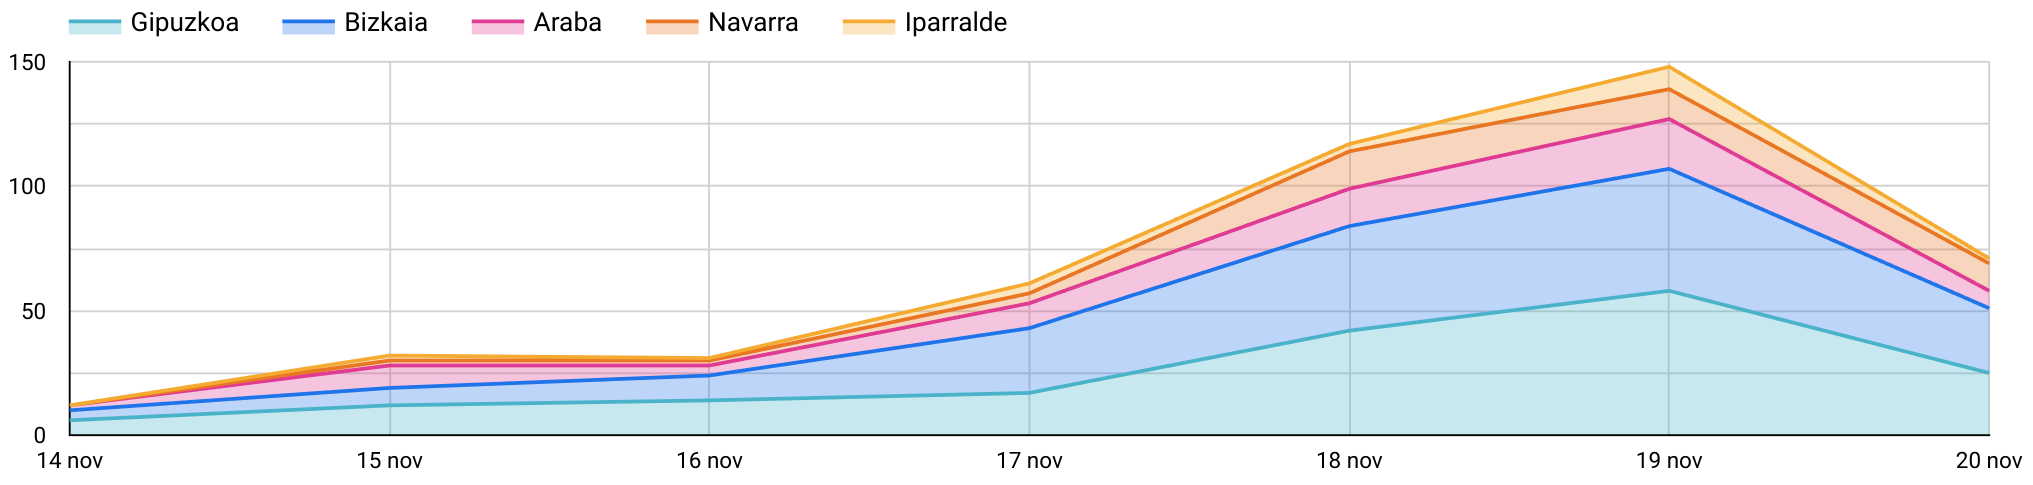
\includegraphics[width=0.9\linewidth]{img/semana.png}
\end{center}


\subsection{Futuros eventos}

Para la última sección se ha decidido crear distintos filtros para que sólo aparezcan eventos que están registrados que se van a celebrar en el futuro y diferenciando idioma.

Se han creado tres filtros:
\begin{itemize}
    \item \textbf{Filtro castellano}: Para la gráfica que sólo muestra eventos que se han especificado que van a ser en castellano.
    \item \textbf{Filtro Euskera}: Para la gráfica que sólo muestra eventos que se han especificado que van a ser en euskera.
    \item \textbf{Filtro futuros}: Que sirve para que las gráficas de esta sección sólo incluyan eventos cuya fecha de inicio sea mayor o igual que el 10 de Noviembre.
\end{itemize}

\begin{center}
    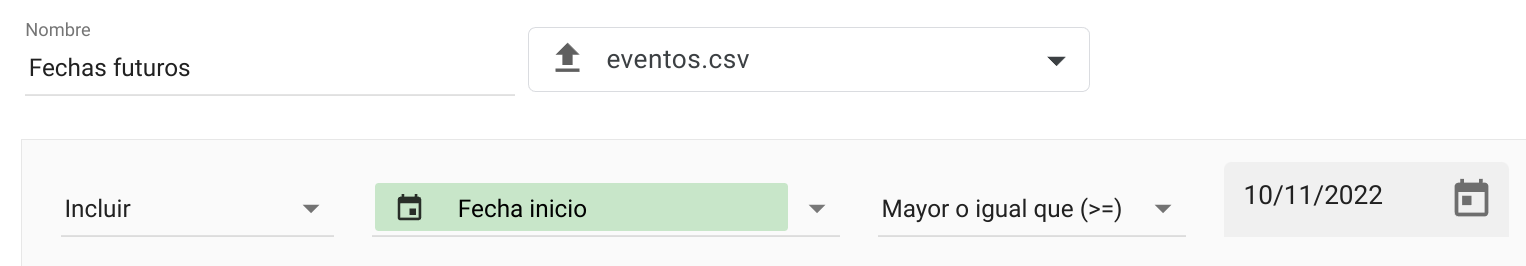
\includegraphics[frame,width=0.9\linewidth]{img/futuro.png}
\end{center}

De esta manera, y aplicando los filtros, la sección queda:

\begin{center}
    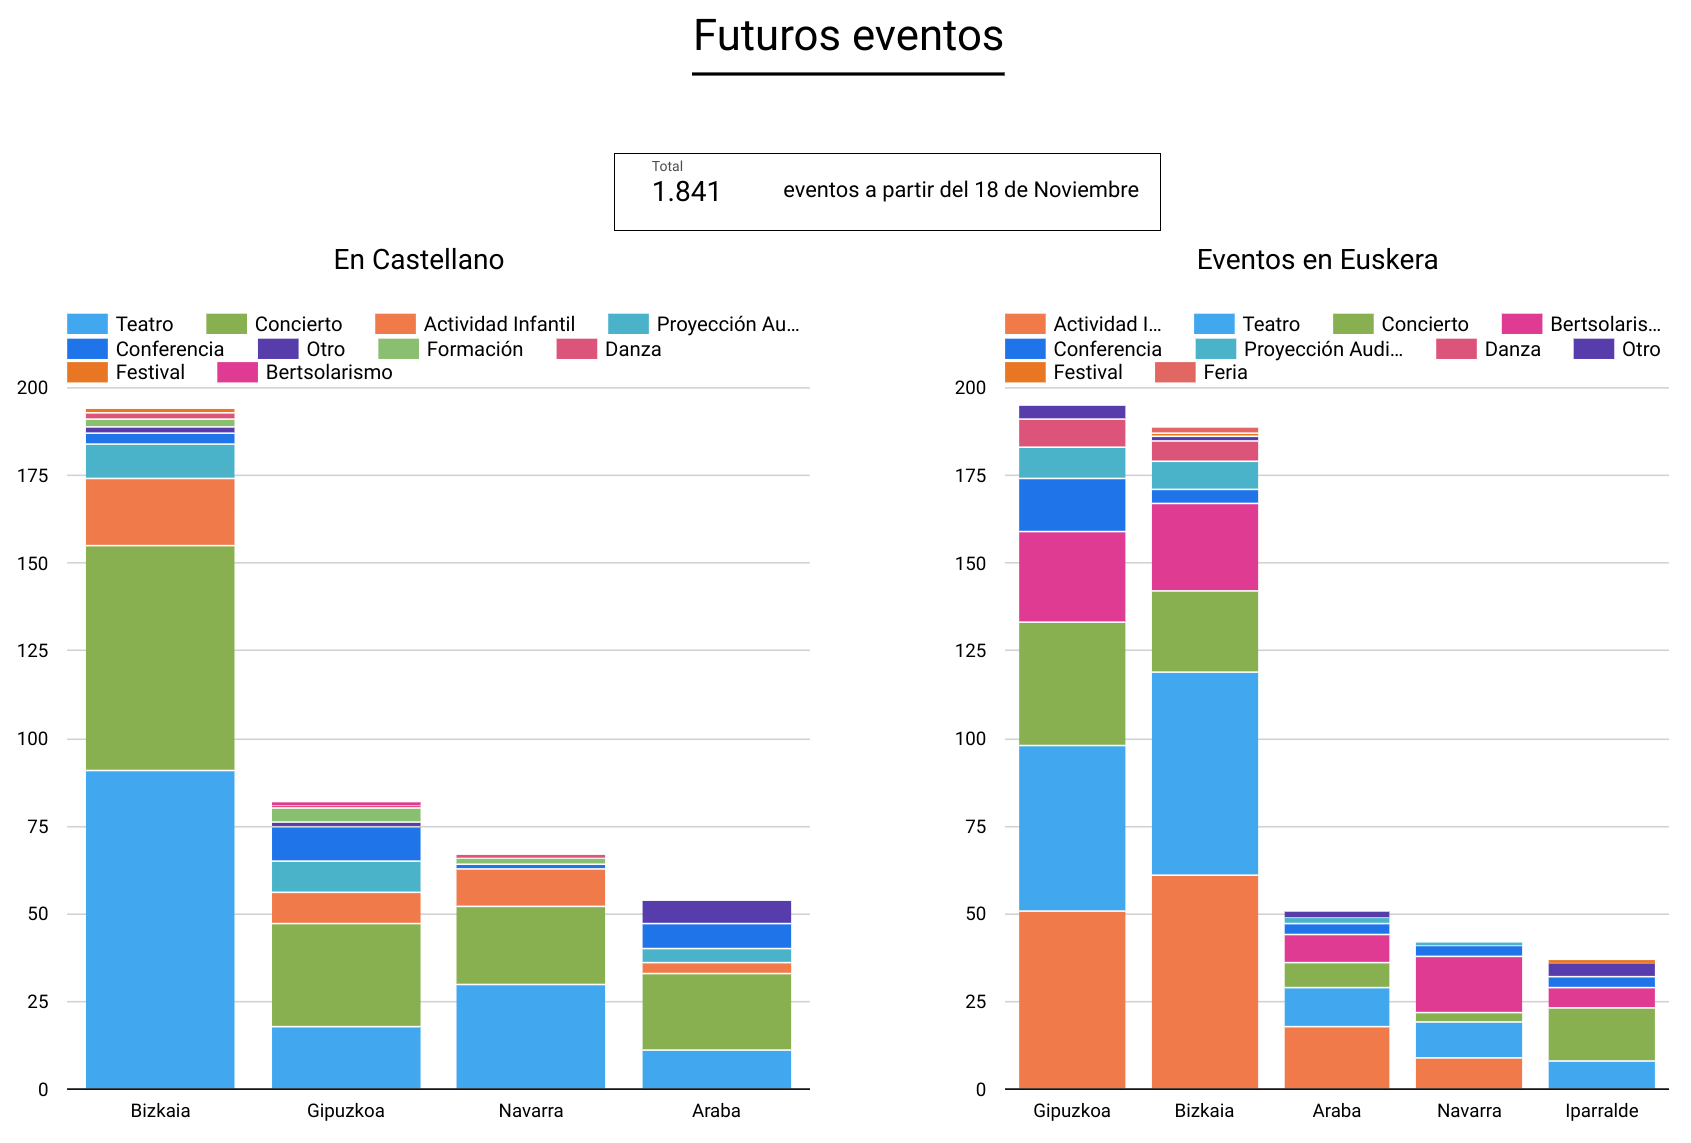
\includegraphics[frame,width=0.9\linewidth]{img/futuro2.png}
\end{center}

Poniendo el ejemplo del gráfico de castellano, contiene dos de los filtros mencionados previamente:

\begin{center}
    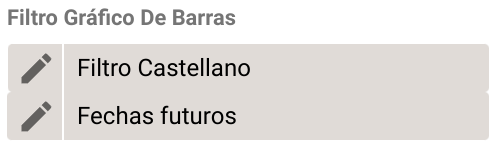
\includegraphics[frame,width=0.4\linewidth]{img/filtros.png}
\end{center}


\chapter{Conclusiones}

A l


\end{document}
